\documentclass[a4paper, 12pt]{article}

\usepackage{graphicx}
\usepackage[font=small, labelfont=bf, labelsep=colon]{caption}
\usepackage{amsmath, amssymb}
\usepackage{float}
%\usepackage{textcomp}
%\usepackage{siunitx}
\usepackage[dvipsnames]{xcolor}
%\usepackage{ctable}
%\usepackage{multirow}
\usepackage[flushmargin, bottom]{footmisc} 
\usepackage{hyperref}

%\hypersetup{
%colorlinks = true,
%linkcolor = {blue!80!black}
%}

\graphicspath{{../../Code_and_Pics/Pictures/}}

%%%%%%%%%%%%%%%%%%%%%%%%%%%%%%%%%%%%%%%%%%%%%%%%%%%%%%%
% Layout parameters 
\setlength{\parindent}{0em}
\setlength{\parskip}{2ex}
\linespread{1.2}

\renewcommand{\floatpagefraction}{.99} % Minimum fraction of floats, in a page that has only floats. Only figures taking up more than that will get their own page. Default 0.5
\renewcommand{\topfraction}{0.99}  % Maximum fraction of page for floats at top. I.e.: floats taking up more than this will have no text below. Default: 0.7.
\renewcommand{\textfraction}{0.01} % Minimum fraction of page that must have text (otherwise, the page will only have float). Default: 0.2 

\addtolength{\textwidth}{2cm}
\addtolength{\hoffset}{-1cm}
\setlength{\topmargin}{-1cm}
\addtolength{\textheight}{1cm}

\setlength{\skip\footins}{6mm} % space between end of text and horizontal line of footnote
\setlength{\footnotesep}{5mm} % space between footnote line and first entry, and between consecutive entries of footnote



%%%%%%%%%%%%%%%%%%%%%%%%%%%%%%%%%%%%%%%%%%%%%%%%%%

%%%%%%%%%%%%%%%%%%%%%%%%
%%%%% NEW COMMANDS
%%%%%%%%%%%%%%%%%%%%%%%%

% Text commands
\newcommand{\spc}{1ex}
\newcommand{\eg}{\textit{e.g.}}
\newcommand{\ie}{\textit{i.e.}}
\newcommand{\red}{\textcolor{red}}

% Maths Commands



%%%%%%%%%%%%%%%%%%%%%%%%%%%%%%%%%%%%%%%%%%%%%%%%%%%%%

\title{(Very!) Preliminary Report - ColaLife Project}

\author{}
\date{}

\begin{document}

\maketitle

The following is a draft upon which to develop the Methods and Results sections of the paper. As it stands, it assumes that the context and the data have already been introduced.

\section{Methods}

\subsection{Analyses on the Aggregated Data}
%Our data reports how each case of diarrhoea was treated in each of seven different health centres, both before and after co-packaging became available. the number of diarrhoea cases
The present study aims to investigate whether the co-pack introduction has significantly increased the chance with which an under-five child affected by diarrhoea is prescribed both ORS and zinc as treatment. After a brief introduction of the statistical framework and notation used throughout the work, in this section we present the tools and analyses employed to address the above question.  

{\footnotesize \red{(I wrote the following paragraph with the goal of giving context to everything that follows and thus to make things as clear as possible. I feel that a concept such as the one highlighted below -- \textit{i.e.}, that a given quantity (such as $p_1$ or $p_2$) is intrinsically unknown, and the data is just a way to \emph{estimate} it -- may not be so obvious to a non-statistician. That's why I wrote the paragraph, although I guess many authors would gloss over such clarifications. Happy to hear your opinion when we talk.)}}


The main quantity of interest throughout this work is the probability with which an under-five child, presented to an health centre for diarrhoea treatment\footnote{Of course, truthfulness of this to be checked.}, is treated correctly (\textit{i.e.}, with both ORS and zinc).
%To allow for the possibility that this probability has changed, in any direction, after the introduction of the co-pack,
To allow for the possibility of a change in the value of this probability following the co-pack introduction, 
 we denote by $p_1$ its value before the co-pack introduction, and by $p_2$ its value after the co-pack introduction. 
Although both probabilities are unknown, the available data can be employed to estimates them and their difference/ratio with a given confidence, and more generally to carry out statistical analyses to address the question that $p_2>p_1$ (\textit{i.e.}, that the co-pack introduction has increased the probability of correct treatment).

Either of $p_1$ and $p_2$ can be estimated as the proportion of correctly-treated children (CTC) within the appropriate sample. To quantify the reliability of the estimate, we include a $95\%$ confidence interval (CI), computed via the Clopper-Pearson method for an exact binomial CI \cite{clopper1934}. The interval is expected to contain the true probability $p_i$ with 95\% confidence.

To test whether a significant increase in such proportion has taken place upon introduction of the ORS and zinc co-pack, we perform a one-sided test of homogeneity of binomial proportions. This tests the null hypothesis that the proportions of CTC before co-pack introduction and after co-pack introduction are equal to each other ($p_1=p_2$), against the alternative that the latter is higher than the former ($p_2>p_1$).
This and all other tests of this work are performed at the $5\%$ significance level: 
that is, the null hypothesis is rejected whenever the $p$-value $<0.05$.
%in other words, a $p$-value $<0.05$ leads to rejecting the null hypothesis.
%\footnote{I guess we could introduce an acronym for the ``proportion of correctly treated children'', since this is the main quantity the whole work focuses on.} has taken place after co-packaging introduction.

The above choice of significance level coincides with the most commonly adopted choice across the applied statistics literature, both in medicine and beyond. However, we wish to stress that the $5\%$ choice is merely a convention. Two $p$-values such as, \eg, $p=0.049$ and $p<0.0001$, are both significant at the $5\%$ level. 
Nonetheless, the level of evidence that they carry against the null hypothesis (and in favour of the alternative) is very different. A $p$-value $<0.0001$ reveals that, under the null hypothesis, the observed data has a chance of happening lower to one in ten thousand. This clearly represents a much stronger evidence against the null hypothesis than if the data could happen in about one every twenty cases ($p\approx 0.05$) under the null hypothesis.\footnote{We can discuss whether similar considerations/explanations should be included. I feel they can have value since people may not be really familiar with statistical tests or interpretation of $p$-values, but we'll discuss this together with all the rest in a call.}

The p-value of the afore-mentioned homogeneity of proportions test is a purely measure of statistical significance. As such, it does provide a quantitative measure of the effect of co-packaging introduction on the proportion of CTC. To quantify this, we employ i) the difference between the two proportions, and ii) the rate ratio.

The difference between the two proportions is estimated via the sample difference and the $95\%$ Wald CI \cite{agresti2002}. The interval is constructed using the large-sample normal approximation and provides a range of values that are expected to contain the true difference of the two proportions, with 95\% confidence. 
The rate ratio is instead computed as the ratio between the proportions of CTC after co-pack introduction, and the proportion before co-pack introduction. It quantifies how many times more (or less) likely a child is to be correctly treated from diarrhoea after the co-pack introduction, than before. A CI for the rate ratio is provided, following the method in \cite{agresti2002, nam1995}.


\subsection{Logistic Model}



\section{Results}

{\small \it \red{As mentioned in the project proposal, I plan to divide the Results (as well as the Methods) section into two parts: one which only looks at the agglomerated data, and one which instead considers how this agglomerated data is spread across the seven centers. The methods and results section on this Part2 are being written.}}

\subsection{Analyses on the Agglomerated Data}
{\bf \underline{The row data (to be summarised in a table..)}}\\[1ex]
% The data in Table ** summarises the number of total diarrhoea cases presented....
Before the co-pack introduction, a total of 176 cases of diarrhoea were recorded across the seven centres, of whom 77 were given both ORS and zinc (11 of these cases where given less than ten zinc tablets though).
\\
After the co-pack introduction, 389 total cases were instead recorded across the seven centres, of whom 337 were correctly treated (all of whom with at least ten zinc tablets). This leads to the following results.

Before co-pack, we estimate the probability of correct treatment as $0.44$, CI: $(0.36, 0.51)$. After co-pack, the estimate rises $0.87$, CI: $(0.83, 0.90)$.
{\it \footnotesize Note that the ``before'' estimate is computed by also classifying as correctly treated those children who were given less than 10 zinc tablets. Otherwise, the estimate becomes 0.38 with a CI of (0.30, 0.45).}
Moreover, a one-sided test of homogeneity of proportions returns a highly significant $p$-value ($p<0.0001$), suggesting that the data carries strong evidence towards the hypothesis that the proportion of CTC has increased after introduction of the co-pack.
The difference between the two proportion is estimated to be $0.43$, with a 95\% CI of $(0.35, 0.51)$.

Figure~\ref{Fig_Overall_Proportions} provides a graphical illustration of the above numbers.
The left panel shows the two proportions (bars) and their CIs (whiskers) on a percentage scale, while the right panel highlights the position of the 95\% CI of their difference, on a scale -100\% to 100\%.
It can be noticed that the CIs for the two proportions are neatly separated from each other, suggesting that the possibility that the true proportions are equal ($p_1=p_2$) is extremely remote. This is additionally confirmed by the 95\% CI of their difference, which lies entirely within the positive side of the range.\footnote{I put a small note here, something to briefly discuss in the call.}

% positive values signify that a significant increase....





\begin{figure}
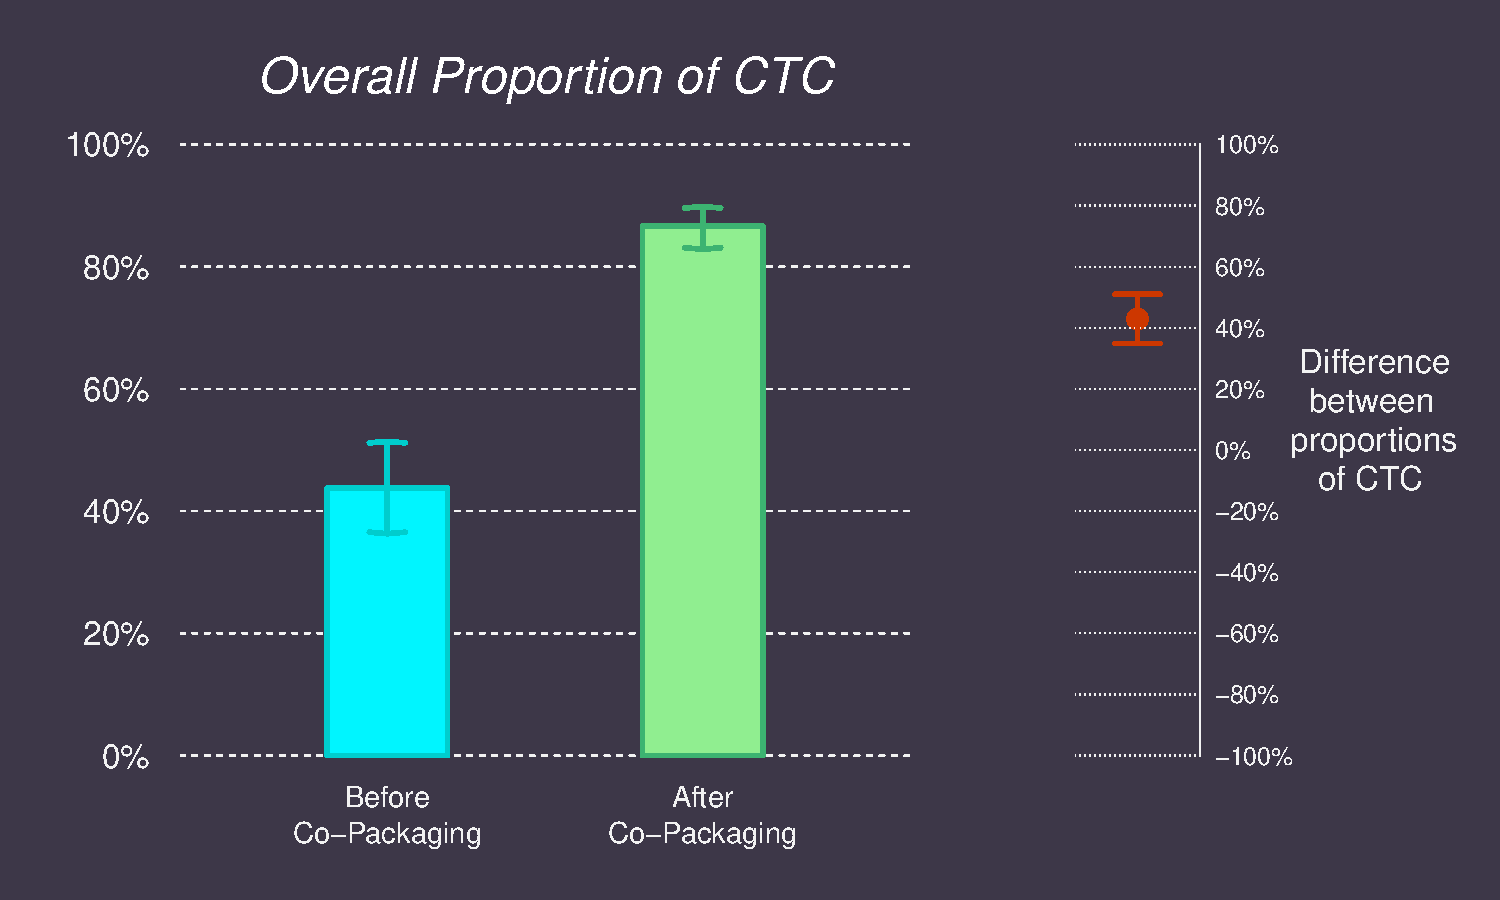
\includegraphics[width=\textwidth]{Overall_Difference_Proportions}
\caption{Comparison of the proportion of CTC across all seven centres, before and after co-packaging. 
Left panel: Each of the two proportions is shown as the height of the corresponding bar, with 95\% CI (whiskers). Right panel: CI of the difference between the two proportions.}
\label{Fig_Overall_Proportions}
\end{figure}

Finally, the 95\% CI for the rate ratio of the two proportions equals $(1.68, 2.37)$. 
In other words, with 95\% confidence, we can state that
the rate at which a child is correctly treated from diarrhoea has become between $68\%$ and $137\%$ higher after the introduction of the co-pack, than it was before.
The 99\% CI $(1.61, 2.52)$ is only slightly wider and once again entirely confined within the region of numbers greater than one (mirroring an increase of the probability of correct treatment).

%%%%%%%%%%%%%%%%%%%%%%%%%%%%%%%%%%%%%%%%

%%%%%%%%%%%%%%%%%%%%%%%%%%%%%%%%%%%%%%%%


\subsection{Analyses on the Single Centres}
Similarly to the analysis performed on the agglomerated data, we can compute the proportions of CTC and their CIs for each of the seven centres, before and after the co-pack introduction. 
Figure~\ref{Fig_Single_Proportions} provides an illustration of the comparison.

As in Figure~\ref{Fig_Overall_Proportions}, the height of each bar represents the sample proportion of CTC\footnote{We may consider to introduce earlier a unique acronym for the ``Proportion of correctly-treated children'', since this is the main quantity of interest throughout the work.} in a specific context, that is, for a given centre and either before or after introduction of the co-pack. Associated with the sample proportion is the 95\% CI quantifying the reliability of the estimate.

We note that the increase in the proportion of CTC concerns every one of the seven centers, 
%a stronger result than the one shown by Figure~\ref{Fig_Overall_Proportions} which instead concerned the agglomerated data.
not just agglomerated data as shown in Figure~\ref{Fig_Overall_Proportions}.
The amplitude of the CIs varies considerably between centres, reflecting the different sample sizes available in different centres: larger sample sizes yield narrower CIs. 
For all centres except Mulawbwa, the CIs before and after co-pack do not overlap with each other. This is a strong indication that a significant increase in the proportion of CTC has taken place in those centres after the co-pack introduction. Mulawbwa is the only center for which a slight overlap between the two CIs can be observed. Nonetheless, the 95\% CI for the difference of proportions in this centre is anyway confined within the positive range $(0.014, 0.257)$, which indicates that -- even for this centre -- we are more than 95\% confident that the proportion of CTC has significanly increased after the co-pack introduction.
 
 Comment can be inserted on the fact that Mulabwa HC differentiate itself quite notably from the other centers. For example, before co-pack it already exhibited a percentage of CTC around 70\%, while all other seven centers exhibit a percentage lower than 40\%. The proportion of CTC after is instead mostly in line with the other centers. 
 

\begin{figure}
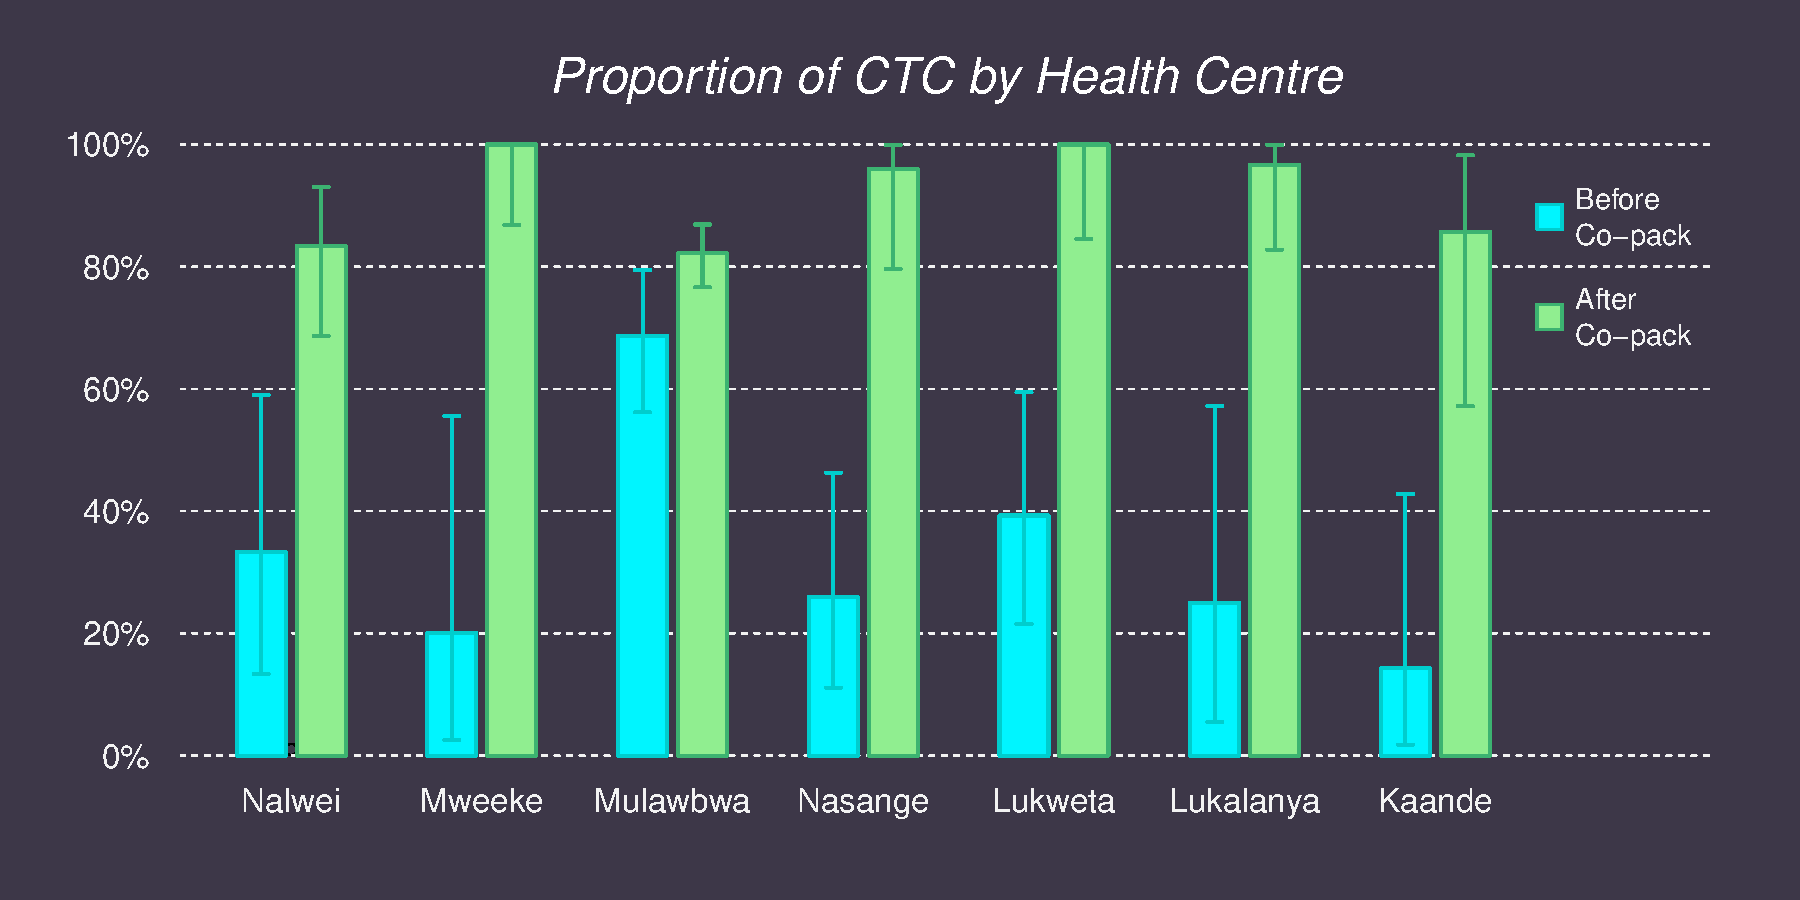
\includegraphics[width=\textwidth]{HC_Proportions}
\caption{Comparison of the proportion of CTC before and after co-packaging, for each of the seven health centres. The sample proportion in each case is represented by the height of each bar, while the whiskers identify the associated 95\% CI.}
\label{Fig_Single_Proportions}
\end{figure}






\newpage
\bibliographystyle{unsrt} 
\bibliography{References}  


\end{document}
